\documentclass{article}

\usepackage{mmacells}

\usepackage{pandekten}
\usepackage{dashrule}

\usepackage[compat=1.1.0]{tikz-feynman}

%workaround from link
\usetikzlibrary{external}
\immediate\write18{mkdir -p pgf-img}
\tikzexternalize[
  prefix=pgf-img/,
  system call={
    lualatex \tikzexternalcheckshellescape -halt-on-error -interaction=batchmode -jobname="\image" "\texsource" || rm "\image.pdf"
  },
]

\makeatletter
\newcommand*{\shifttext}[1]{%
  \settowidth{\@tempdima}{#1}%
  \hspace{-\@tempdima}#1%
}
\newcommand{\plabel}[1]{%
\shifttext{\textbf{#1}\quad}%
}
\newcommand{\prule}{%
\begin{center}%
\hdashrule[0.5ex]{.99\linewidth}{1pt}{1pt 2.5pt}%
\end{center}%
}

\makeatother

\newcommand{\minusbaseline}{\abovedisplayskip=0pt\abovedisplayshortskip=0pt~\vspace*{-\baselineskip}}%

\setlength{\parindent}{0pt}

\title{Assignment 4}
\author{Ze Chen}

\begin{document}

\maketitle

\plabel{1}%
We denote for short
\[ \lambda(\vb{x}) = \lambda e^{-\abs{\vb{x}}^2/L^2}. \]
Then
\begin{align*}
    \bra{0}\ket{\lambda} &= \frac{\displaystyle\int \mathcal{D}\phi \exp[\int \dd[d+1]{x} \qty(\frac{1}{2}\phi\qty(-i\partial_t^2 + i\grad^2)\phi - i\lambda(\vb{x})\delta'(t)\phi)]}{\displaystyle \int \mathcal{D}\phi \exp[\int \dd[d+1]{x} \qty(\frac{1}{2}\phi\qty(-i\partial_t^2 + i\grad^2)\phi)]} \\
    &= \exp\qty[\frac{i}{2} \left< \lambda \delta'_0, \frac{1}{\partial_0^2 - \grad^2+i\epsilon} \lambda \delta'_0 \right>] \\
    &= \exp[\frac{1}{2} \int \frac{\dd[d]{\vb{k}}}{(2\pi)^d} \int \frac{\dd{\omega}}{2\pi i} \frac{\omega^2}{\omega^2 - \abs{\vb{k}}^2 + i\epsilon}\lambda^2(\vb{k})] \\
    &= \exp[-\frac{1}{4} \int \frac{\dd[d]{\vb{k}}}{(2\pi)^d} \abs{\vb{k}} \lambda^2(\vb{k})] \\
    &= \exp[-\frac{1}{4} \frac{L^d}{L} \int \frac{\dd[d]{(L\vb{k})}}{(2\pi)^d} \abs{L\vb{k}} \pi^{d} e^{-\abs{L\vb{k}}^2/2}] \\
    &= \exp[-L^{d-1} \cdot I(d)].
\end{align*}
For $d>1$, $\bra{0}\ket{\lambda} \rightarrow 0$ as $L\rightarrow \infty$, while for $d=1$, $\bra{0}\ket{\lambda} \neq 0$.
Therefore $d>1$ for spontaneous symmetry breaking to occur.

\prule

\plabel{2 (a)}%
Let
\[ z(\sigma_0,\sigma_3) = \sum_{\sigma_1}\sum_{\sigma_2} \exp[\beta J_0(\sigma_0 \sigma_1 + \sigma_1 \sigma_2 + \sigma_2 \sigma_3)]. \]
Then
\[ z(1,1) = z(-1,-1) = e^{3\beta J_0} + 3e^{-\beta J_0} = e^{\beta J_1 + c}, \]
and
\[ z(1,-1) = z(-1,1) = 3e^{\beta J_0} + e^{-3\beta J_0} = e^{-\beta J_1 + c}. \]
Therefore,
\begin{align*}
    \beta J_1 &= \frac{1}{2} \log(\frac{3e^{-\beta J_0} + e^{3\beta J_0}}{e^{-3\beta J_0} + 3e^{\beta J_0}}), \\
    c &= \frac{1}{2}\log[(e^{-3\beta J_0} + e^{\beta J_0})(3e^{3\beta J_0} + e^{3\beta J_0})].
\end{align*}

\plabel{(b)}%
Since $\abs{\beta J_1} < \beta J_0$, we have $J_n \rightarrow 0$ as $n\rightarrow \infty$.
\begin{center}
    \begin{tikzpicture}
        \begin{axis}[domain=-2:2,samples=100,xlabel=$\beta J_0$,ylabel=$\beta J_1$]
            \addplot[dashed] {x};
            \addplot[] {0.5*ln((exp(3*x)+3*exp(-x))/(3*exp(x)+exp(-3*x)))};
            \addplot[mark={}] coordinates {
                (1.54657,1.54657)
                (1.54657,1)
                (1,1)
                (1,0.474396)
                (0.474396,0.474396)
                (0.474396,0.0864155)
                (0.0864155,0.0864155)
                (0.0864155,0.000640527)
                (0.000640527,0.000640527)
            };
        \end{axis}
    \end{tikzpicture}
\end{center}

\prule

\plabel{3}%
In problem 1 of assignment 3 we set both the scalar the fermion mass to zero and renormalize at $p^2 = -M^2$ and find
\begin{align*}
    \delta_{\phi} &= -\frac{4g^2}{(4\pi)^2}\qty(\frac{1}{\epsilon} - \log M), \\
    \delta_\psi &= -\frac{g^2}{(4\pi)^2}\qty(\frac{1}{\epsilon} - \log M), \\
    \delta_g &= \frac{2g^3}{(4\pi)^2}\qty(\frac{1}{\epsilon} - \log M), \\
    \delta_\lambda &= \frac{3\lambda^2 - 48g^4}{(4\pi)^2}\qty(\frac{1}{\epsilon} - \log M).
\end{align*}
Therefore,
\begin{align*}
    \beta_g &= M\pdv{M}\qty(-\delta_g + \frac{1}{2}g \qty(\delta_\phi + 2\delta_\psi)) = \frac{5g^3}{(4\pi)^2} \\
    \beta_\lambda &= M\pdv{M}\qty(-\delta_\lambda + \frac{1}{2}\lambda \qty(4\delta_\phi)) = \frac{3\lambda^2 - 48g^4 + 8\lambda g^2}{(4\pi)^2}.
\end{align*}
\begin{center}
    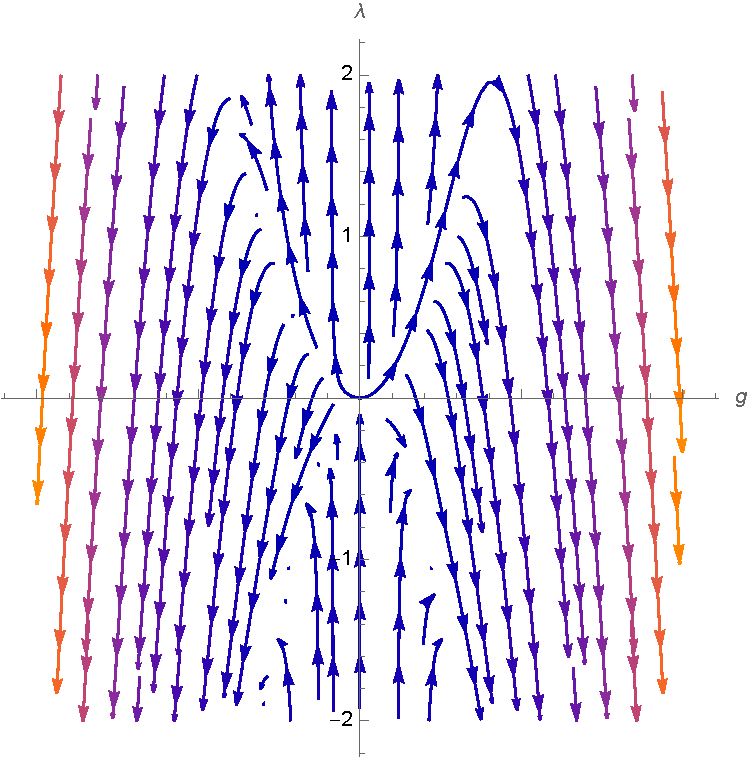
\includegraphics[width=.5\linewidth]{img/HW4.3.pdf}
\end{center}

\end{document}
